\documentclass[main.tex]{article}
\usepackage{subfiles}
\usepackage{hyperref}
\usepackage{csquotes}
\usepackage{amsmath}
\usepackage{amsfonts}
\usepackage[]{geometry}
\usepackage{graphicx}

\graphicspath{{./figures/}}

\begin{document}
    \section[P3: Same \texorpdfstring{$\mu$}{mean} and \texorpdfstring{$\sigma^2$}{variance}]{Same mean and variance for different PDFs}
    Consider the uniform distribution $U$ (same as \ref{eq:unidist})
    \begin{equation}
        U(x;a,b) = \left\{\begin{matrix}
        \frac{1}{b-a} & \textup{if } x \in [a,b] \\
        0 & \textup{otherwise}
        \end{matrix}\right.
    \end{equation}
    Consider the normal distribution $N$ given by
    \begin{equation}
        \label{eq:normal}
        N(x; \mu, \sigma^2) = \frac{1}{\sqrt{2\pi \sigma^2}} \; \mathrm{exp} \left( -\frac{(x-\mu)^2}{2\sigma^2} \right )
    \end{equation}
    As observable, the normal distribution is explicitly parameterized by mean $\mu$ and variance $\sigma^2$, whereas the uniform distribution has mean $\mu_U = \frac{a+b}{2}$ and variance $\sigma_U^2 = \frac{(b-a)^2}{12}$ (as proven by \ref{eq:unidist-varproof}). \par
    We can select any $a$ and $b$ for a uniform distribution (as long as $b>a$), calculate the mean and variance, and then create a corresponding normal distribution. This is shown in Figure \ref{fig:sm-mean-var}.
    \begin{figure}[h]
        \centering
        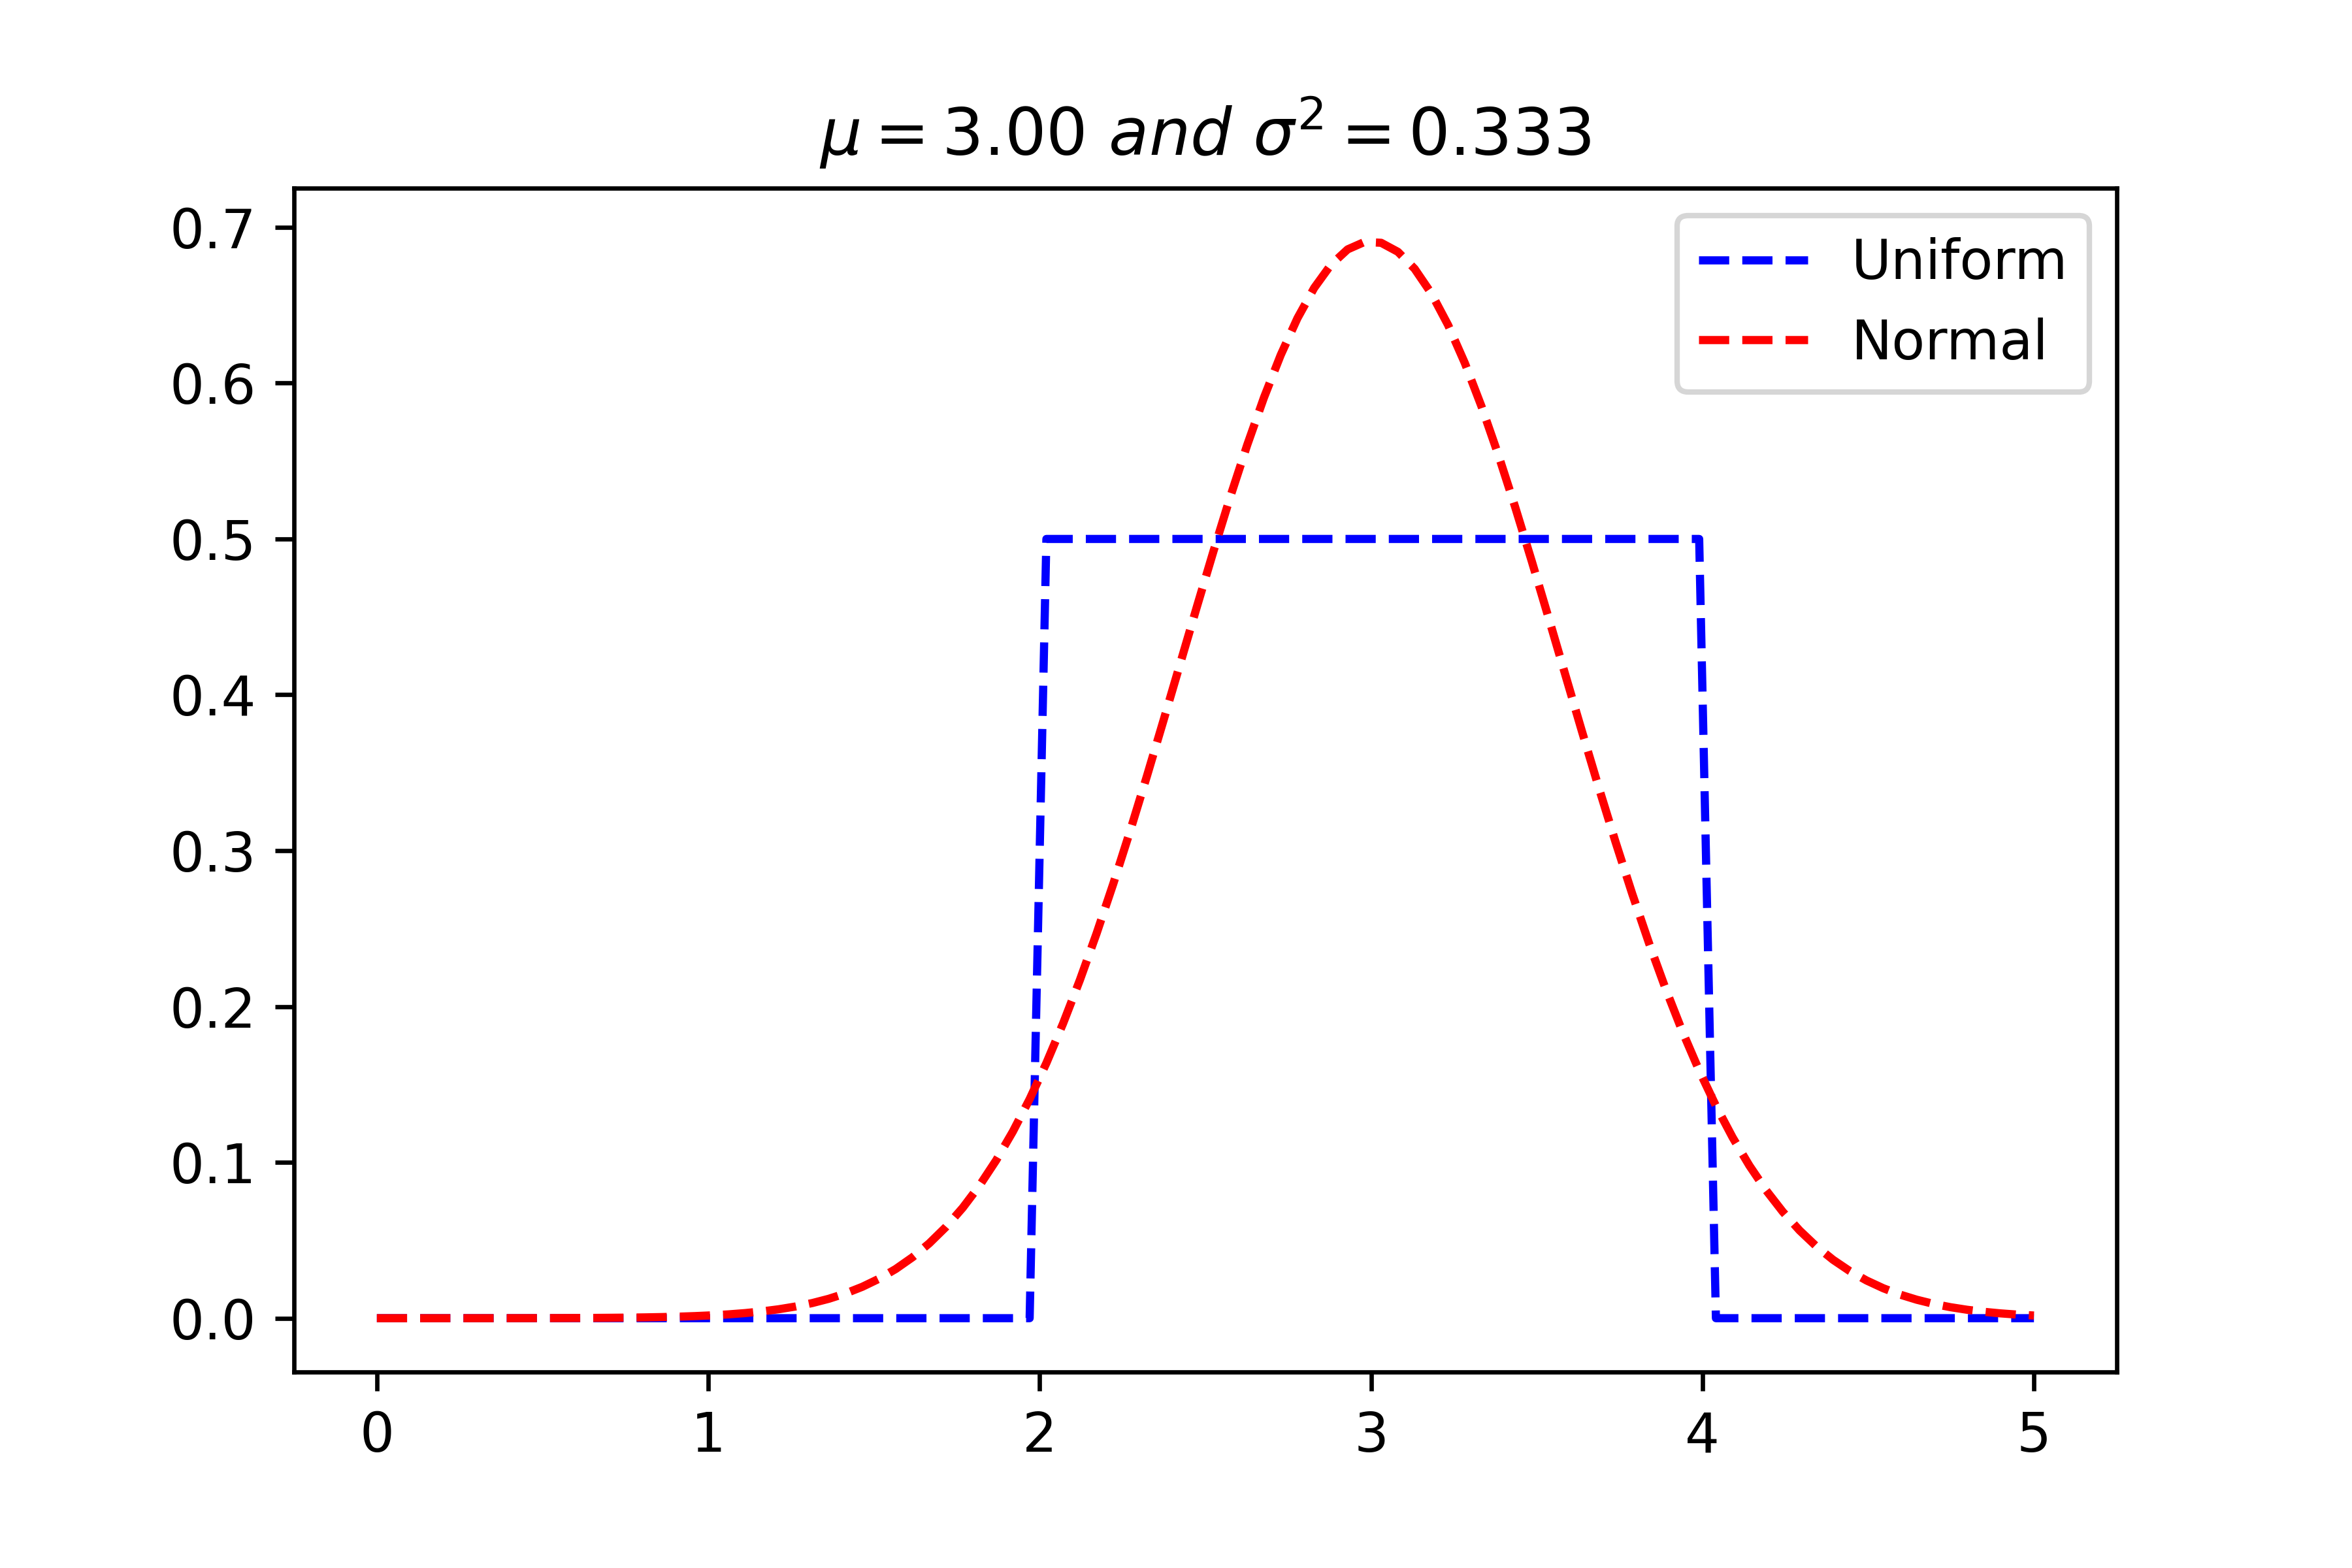
\includegraphics[width=0.7\textwidth]{plot_p3.png} \\
        \caption[Two PDFs with same \texorpdfstring{$\mu$}{mean} and \texorpdfstring{$\sigma^2$}{variance}]{Normal and Uniform distribution having the same mean and variance}
        \small The blue line is for a uniform distribution with $a=2$ and $b=4$. The red line is for a normal distribution with $\mu=3$ and $\sigma^2 = \frac{1}{3}$
        \label{fig:sm-mean-var}
    \end{figure}
    The code responsible for this figure is described in appendix \ref{app:code-p3}.
\end{document}
